\iffalse
\let\negmedspace\undefined
\let\negthickspace\undefined
\documentclass[journal,12pt,twocolumn]{IEEEtran}
\usepackage{cite}
\usepackage{amsmath,amssymb,amsfonts,amsthm}
\usepackage{algorithmic}
\usepackage{graphicx}
\usepackage{textcomp}
\usepackage{xcolor}
\usepackage{txfonts}
\usepackage{listings}
\usepackage{enumitem}
\usepackage{mathtools}
\usepackage{gensymb}
\usepackage{comment}
\usepackage[breaklinks=true]{hyperref}
\usepackage{tkz-euclide} 
\usepackage{listings}
\usepackage{gvv}                                        
\def\inputGnumericTable{}                                 
\usepackage[latin1]{inputenc}                                
\usepackage{color}                                            
\usepackage{array}                                            
\usepackage{longtable}                                       
\usepackage{calc}                                             
\usepackage{multirow}                                         
\usepackage{hhline}                                           
\usepackage{ifthen}                                           
\usepackage{lscape}

\newtheorem{theorem}{Theorem}[section]
\newtheorem{problem}{Problem}
\newtheorem{proposition}{Proposition}[section]
\newtheorem{lemma}{Lemma}[section]
\newtheorem{corollary}[theorem]{Corollary}
\newtheorem{example}{Example}[section]
\newtheorem{definition}[problem]{Definition}
\newcommand{\BEQA}{\begin{eqnarray}}
\newcommand{\EEQA}{\end{eqnarray}}
\newcommand{\define}{\stackrel{\triangle}{=}}
\theoremstyle{remark}
\newtheorem{rem}{Remark}
\begin{document}

\bibliographystyle{IEEEtran}
\vspace{3cm}

\title{Probability Assignment}
\author{EE22BTECH11022-G.SAI HARSHITH$^{*}$% <-this % stops a space
}
\maketitle
\newpage
\bigskip
\renewcommand{\thefigure}{\theenumi}
\renewcommand{\thetable}{\theenumi}

Question: Let $X$ be a positive valued continuous random variable with finite mean $\mu$.
If $Y=[X]$, the largest integer less than or equal to $X$, then which of the
following statements is/are true?
\begin{enumerate}[label=(\Alph*)]
\item $\pr{Y \leq \mu} \leq \pr{X \leq \mu}$ for all $\mu \geq 0$
\item $\pr{Y \geq \mu} \leq \pr{X \geq \mu}$ for all $\mu \geq 0$
\item E(X) $<$ E(Y)
\item E(X) $>$ E(Y)
\end{enumerate}
\fi
\solution Given that $X$ is a positive valued random variable and $Y=[X]$.So,
\begin{align}
X&=Y+Z
\end{align}
Here, $Z$ is an uniform distrubtion.
\begin{align}
Z &\sim U[0,1)\\
F_Z(x)&=x\\
E(Z)&=\frac{1}{2}
\end{align}
Consider
\begin{enumerate}
\item 
\begin{align}
\pr{Y \leq \mu}&=\pr{X-Z \leq \mu}\\
&=\pr{Z \geq X-\mu}\\
&=E(1-F_Z(X-\mu))\\
&=E(1-X+\mu)\\
&=1-E(X)+\mu\\
&=1
\end{align}
From option (A), we have $1 \leq \pr{X \leq \mu}$. Option (A) is wrong since probability can't be greater than 1.
\item
\begin{align}
\pr{Y \geq \mu}&=\pr{X-Z \geq \mu}\\
&=\pr{Z \leq X-\mu}\\
&=E(F_Z(X-\mu))\\
&=E(X-\mu)\\
&=E(X)-\mu\\
&=0
\end{align}
 From option B, we have $\pr{X \leq \mu} \geq 0$. Option (B) is correct.
 \item
\begin{align}
E(Y)&=E(X-Z)\\
&=E(X)-E(Z)\\
&=\mu-\frac{1}{2}\\
&=E(X)-\frac{1}{2}
\end{align}
$E(X) > E(Y)$. Option (D) is correct and (C) is wrong.
\end{enumerate}
\textbf{Steps for Simulation:}
\begin{enumerate}
\item Taking $n$ samples, Generate n exponential random variable($X$) samples.
\item Generate $n$ samples of $Y=[X]$ by floor to every sample of $X$.
\item Find number of samples of $X$ where $X \leq \mu$ and $X \geq \mu$ and divide with $n$ to get $\pr{X \leq \mu}$ and $\pr{X \geq \mu}$ respectively.
\item Find number of samples of $Y$ where $Y \leq \mu$ and $Y \geq \mu$ and divide with $n$ to get $\pr{Y \leq \mu}$ and $\pr{Y \geq \mu}$ respectively.
\item Sum the $n$ samples of $X$ and $Y$ and divide with $n$ to get $E(X)$ and $E(Y)$.
\end{enumerate}
\begin{figure}[!ht]
\centering
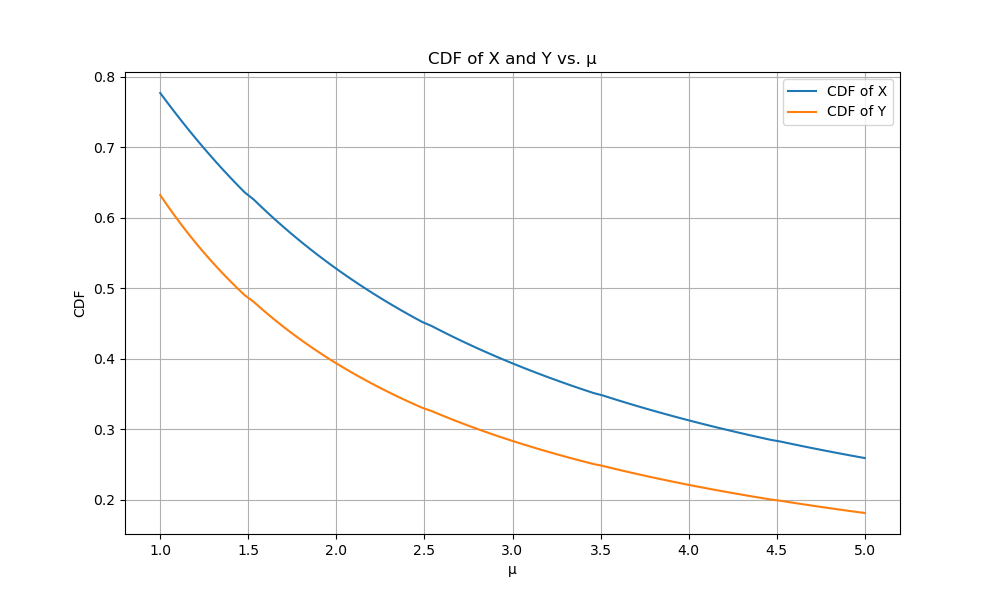
\includegraphics[width=\columnwidth]{figs/figure.png}
\caption{CDF'S of X and Y for varying $\mu$ at x=1.5}
\end{figure}
\textbf{Note:}
At x $\in$ integers, $Y=X$ , so, CDF curves of $Y$ and $X$ are same. At non-integers we can see some difference in CDF curves in $X$ and $Y$.
